
\chapter{�ber das Template}
\label{sec:haupt}

Der Hauptteil kann aus den Kapiteln Aufgabenstellung, Konzept, Implementierung, Test, usw. je nach Arbeitsthema bestehen. innerhalb der \texttt{thesis.tex} wird der Grobaufbau der Arbeit definiert. Die Datei \texttt{header.tex} konfiguriert die Packages und alle Dokumenteigenschaften. Beide Dateien sollten bekannt sein und m�ssen bei Bedarf abge�ndert bzw. erweitert werden. Die LaTeX-Definitionen und die eingebundenen Packages stellen einige M�glichkeiten bereit, diese sollen hier kurz vorgestellt werden.

\section{Sprache}
\label{sec:haupt:lang}

Dieses Dokument kann zur Erstellung von deutschen wie englischen Texten verwendet werden. Die Standardeinstellung ist Englisch, um zu Deutsch zu wechseln m�ssen in den Dateien \texttt{thesis.tex} und \texttt{header.tex} alle mit "`LANGUAGE"' markierten Zeilen entsprechend angepasst werden.

Ein bekanntes Problem ist die nicht immer fehlerfreie Unterst�tzung von deutschen Umlauten. Neben einigen m�glichen Ursachen ist ein oft auftretendes Problem die nicht identische Kodierung der Textdateien innerhalb des Projekts. Treten Probleme nur im Bereich einer \texttt{*.tex} Datei auf muss die Kodierung dieser einen Datei an die der anderen angeglichen werden (z.B. mit Notepad++).

\section{Abbildungen}
\label{sec:haupt:figure}

Das Einbinden von Grafiken soll an Abbildung \ref{fig:beispiel} gezeigt werden. Die Grafik selbst liegt entsprechend der Definition in der \texttt{header.tex} im Projekt-Unterordner "`images"' und sollte zur guten Darstellung als Vektorgrafik oder png-Bilddatei vorliegen.

\begin{figure}[htb]
\begin{center} 
  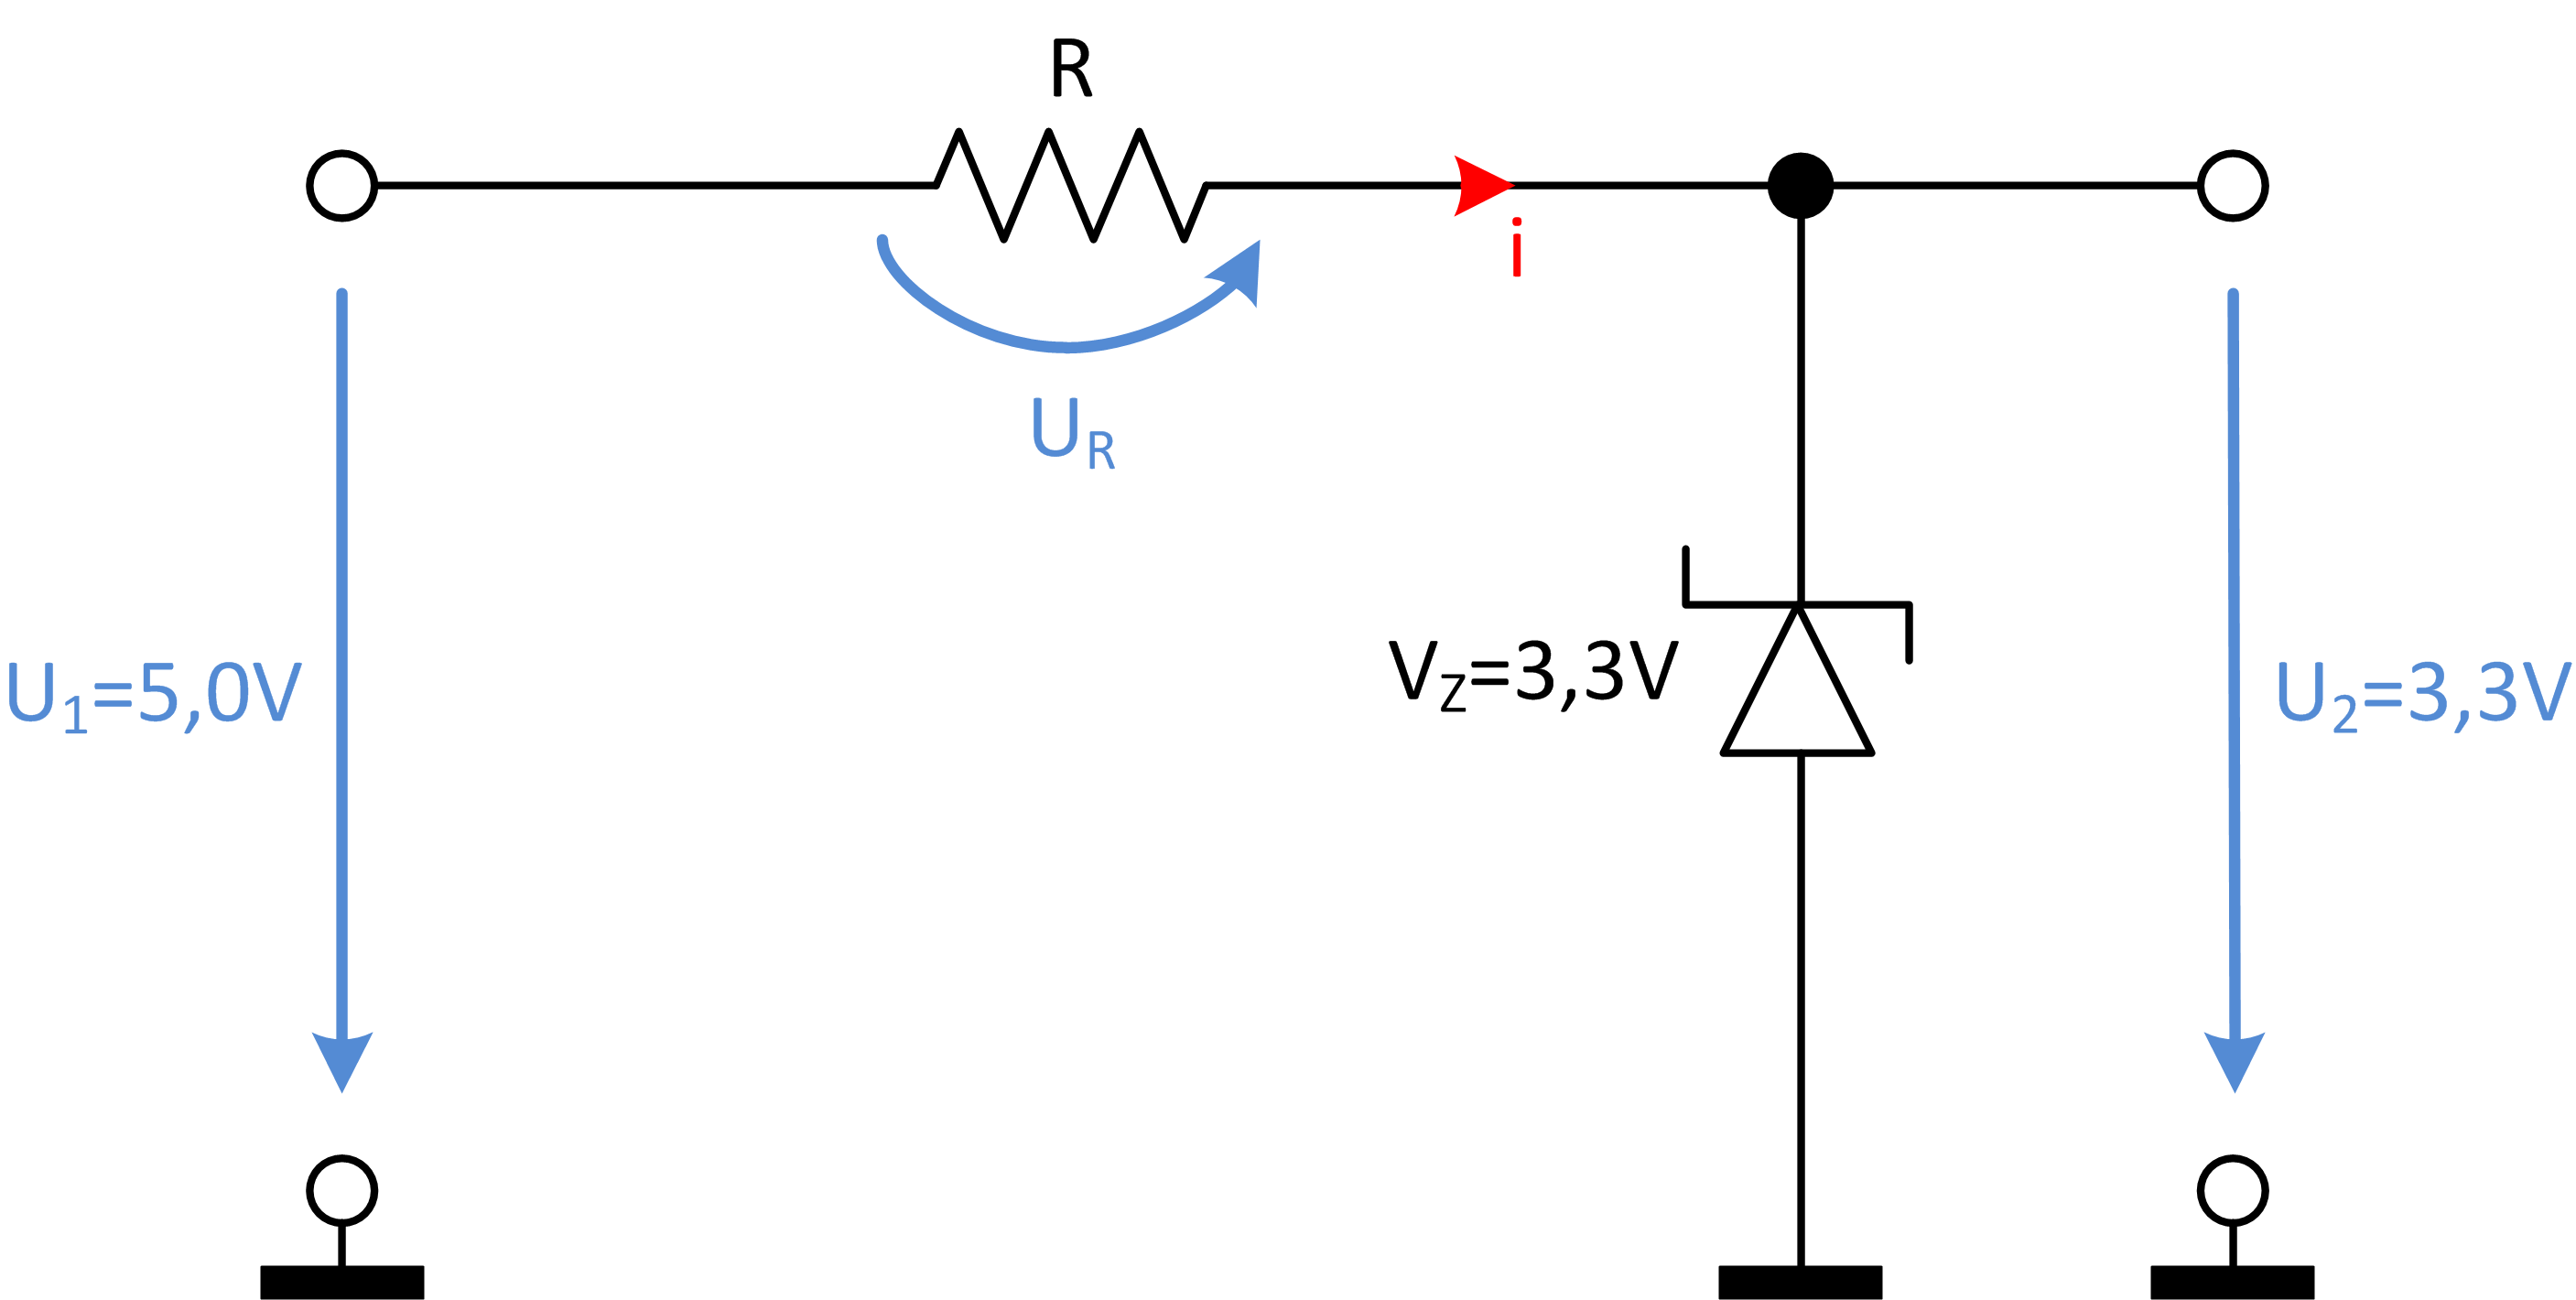
\includegraphics[width=0.40\textwidth]{examplepic}
  \caption{Ein Bild als Beispiel}
  \label{fig:beispiel}
\end{center}
\end{figure}
 
Die Positionsdefinition "`htb"' beschreibt die automatische Positionierung in LaTeX in der bevorzugten Reihenfolge "`here, top, buttom"'. Wenn man wei� was man tut und die Grafik in jedem Fall genau an der gew�hlten Stelle eingebunden werden soll ist "`h!"' zu nutzen. Ein Warning\todoedit{zu beachten}\ wird generiert wenn diese Anforderung nicht erf�llt werden kann.

\section{Verschiedenes}
\label{sec:haupt:misc}

Eine Tabelle unter Nutzung des \texttt{booktabs} Package kann beispielsweise so aussehen:

\begin{table}[htb]
\centering
	\begin{tabular}{llr}
	\toprule
	Device & Teiler & Baudrate [Baud]\\
	\midrule
	\multirow{2}{2.5cm}{Modul Standard}
	 & BR=4 & \num{125000}\\
	 & BR=5 & \num{100000}\\
	\cmidrule{2-3}
	& & Diff=\num{25000}\\
	\addlinespace
	\midrule
	\addlinespace
	\multirow{2}{1.5cm}{Modul ExtendedLong}
	 & Step=0x327 & \num{125033}\\
	 & Step=0x326 & \num{124878}\\
	\cmidrule{2-3}
	 & & Diff=\num{155}\\
	\bottomrule
	\end{tabular}
	\caption{Beispiel Tabelle} 
	\label{tab:bsp}
\end{table}
\todoedit{Beachte dasss hier ein Warning wegen dem zu langen Modulnamen erscheint.}

Quelltext kann mit Hilfe des \texttt{listings} Package direkt oder �ber eine Datei eingebunden werden:

\begin{lstlisting}[caption={\texttt{SCI.c} - SCI-Definitionen}, label=lst:scidefine]
	#define SCIBDH     SCI1BDH
	#define SCIBDL     SCI1BDL
	#define SCIC1      SCI1C1
	#define SCIC2      SCI1C2
	...                ...
\end{lstlisting}

\lstinputlisting[%
		caption=\texttt{wireless\_uart.c} - Auszug,%
		label=lst:scirx,%
		float=hbt,%
		frame={tbrl},%
		%firstline=1,%
		lastline=7,%
]{sourcecode/bsp.c}

Ein Beispiel f�r eine nummerierte Tabelle mit Gro�buchstaben und einer speziellen Formatierung:
\begin{enumerate}[\bfseries (A) {-}]
  \item Das Kapitel \ref{sec:haupt} tr�gt den Titel \nameref{sec:haupt}\footnote{Die Nutzung von Nameref ist in vielen Situationen n�tzlich} und beginnt auf Seite \pageref{sec:haupt} 
  \item \SI{3}{\volt} liegt im Bereich zwischen \SIrange[range-units=single]{2,5}{3,5}{\volt}. Die Stromst�rke wird meist in der Einheit \si{\mA} angegeben und auch eine einfache Zahl wie bspw. \num{65536,128} l�sst sich mit dem Package \texttt{siunitx} sicher darstellen.
\end{enumerate}


\chapter{Introduction} 
\label{ch:Introduction}
A correct design for a system is a crucial step to reach a satisfactory result. Building a model is essential to analyze and evaluate the different possibilities in an early stage, or to prove the correctness of the solution in diverse scenarios. For this purpose, there are several models \cite{zeigler:modsim} that can be used, with different expressiveness and properties. If the model is complex enough, an analytical approach may not be possible due to the need of a complete state space exploration and the state explosion limitation \cite{Valmari1998}. To overcome this problem, simulation methods \cite{simulationmethodsreliability} can provide an acceptable solution but they introduce a new issue: rare-events \cite{goerg:rareevent,Heegaard97speedupsimulation}. If the simulation needs to evaluate a measure \cite{haas:spn} based on an event that is very unlikely to happen (e.g. $10^{-6}$), unless special considerations are taken the simulation will rarely go through this event, therefore a good confidence level will be highly time-consuming to achieve. The goal of the current work is to design, implement and evaluate a simulation algorithm, which will be able to overcome the rare-event limitation without requiring a deep understanding of it, nor a high level analysis of the model. Moreover, it introduces a new concept of how to deal with the simulation execution, avoiding random decisions to achieve an execution as close as possible to an analysis...